\chapter{In-depth Contrastive Error Analysis}
\label{chap:analysis}

% Length
% Graph factors
% Linguistic factors

% Peking: Ensemble method, combination of transition-based and graph-based
% Turku: Support Vector Machines
% Lisbon: A graph algorithm


In this chapter we will examine the results of SemEval-2015 for the Peking, Turku and Lisbon systems described in the previous chapter. The aim of this study is to evaluate the type of errors that state-of-the-art data-driven semantic dependency parsers make. The aim of this comparative analysis is twofold:

\begin{enumerate}
    \item To find differences in the results among a chosen set of parsing systems in order to compare and contrast their strengths and weaknesses.
    \item Empirically identify and verify which types of errors that can be the focus of future research on semantic dependency parsing.
\end{enumerate}

The three systems that we will examine: Peking, Turku, and Lisbon, have been chosen based on two factors:

\begin{enumerate}
    \item They are among the parsing systems with the highest overall scores in SemEval-2015. 
    \item The chosen parsing systems should are based on different algorithms, and include both the local transition-based and global graph-based models that we examined in Chapter \ref{chap:background}.
\end{enumerate}

We will argue that the analysis presented in this chapter can highlight the correlation between the specific types of errors that these parsers make and their theoretical foundation.

In our analysis we take inspiration from a similar study performed by \citeA{McD:Niv:07}, where a comparative analysis of a set of syntactic parsers has been performed. The study focuses on three types of errors: (1) length factors, (2) graph factors, and (3) linguistic factors. We will structure our analysis accordingly, and include a fourth type of errors that examine the multi-classification task of frame predication.

\section{Length factors}

As \citeA{McD:Niv:07} point out, it is well known that syntactic parsing systems have lower accuracy for longer sentences. We observe the same phenomena in the results from SemEval-2015.

\begin{figure}[h]
\caption{Caption}
\centering
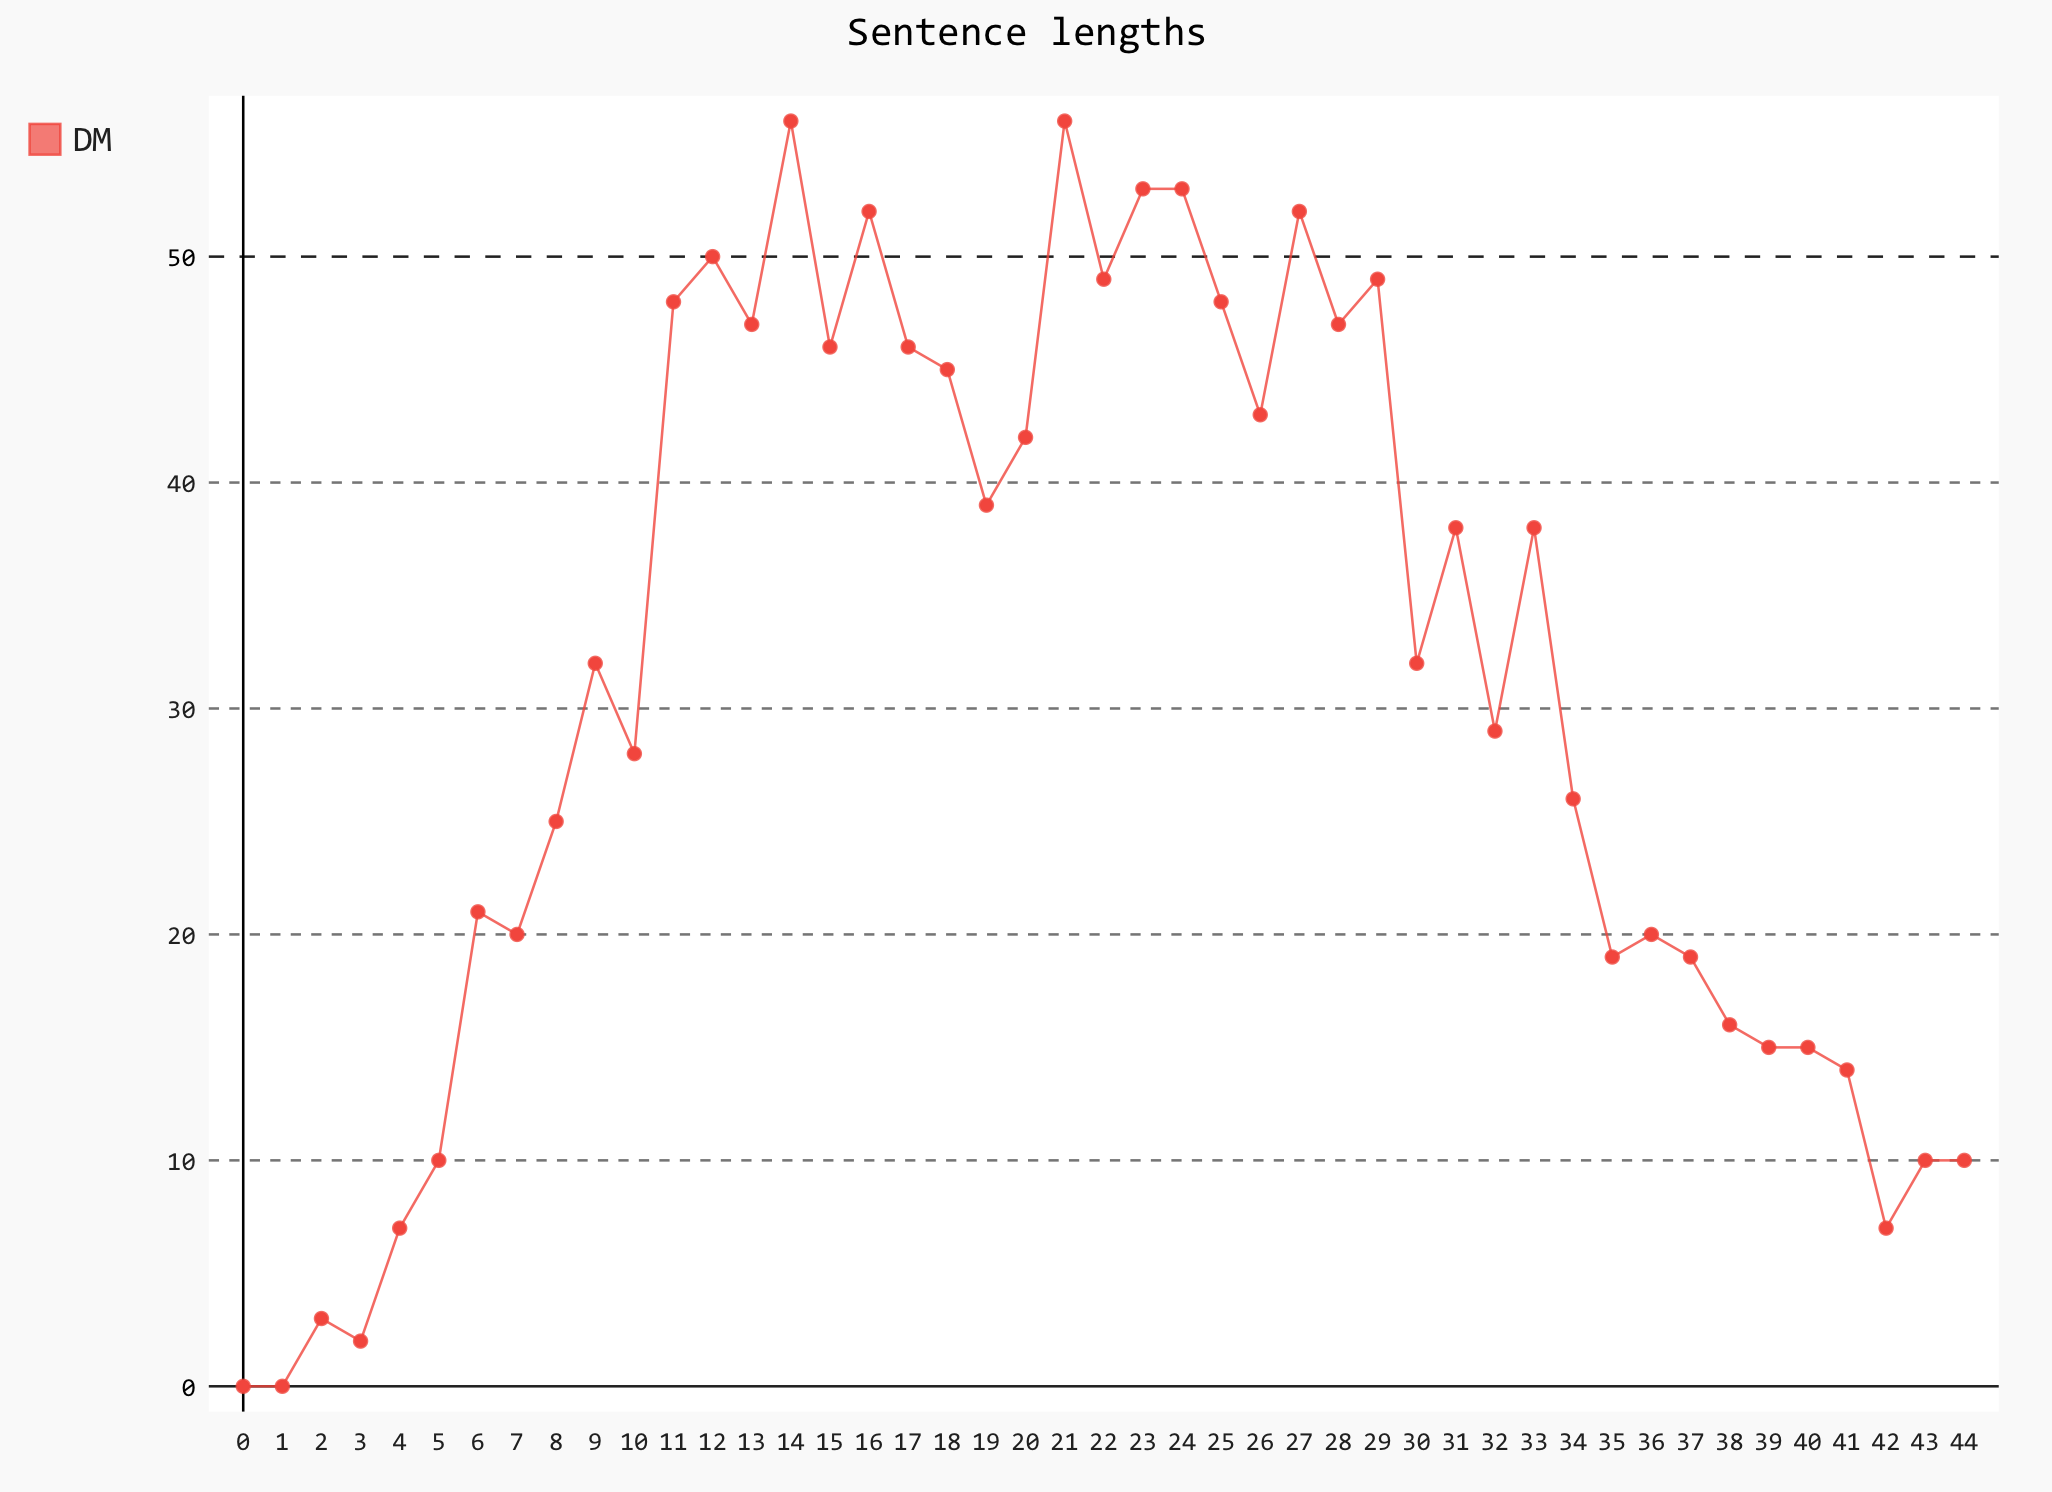
\includegraphics[width=\textwidth]{sentence_length}
\label{fig:sentence_length}
\end{figure}

